\documentclass[crop,tikz]{standalone}
\usepackage{tikz}
\usepackage{amsmath, amssymb}
\usetikzlibrary{arrows,shapes,positioning,shadows,trees,decorations.pathreplacing}

\begin{document}

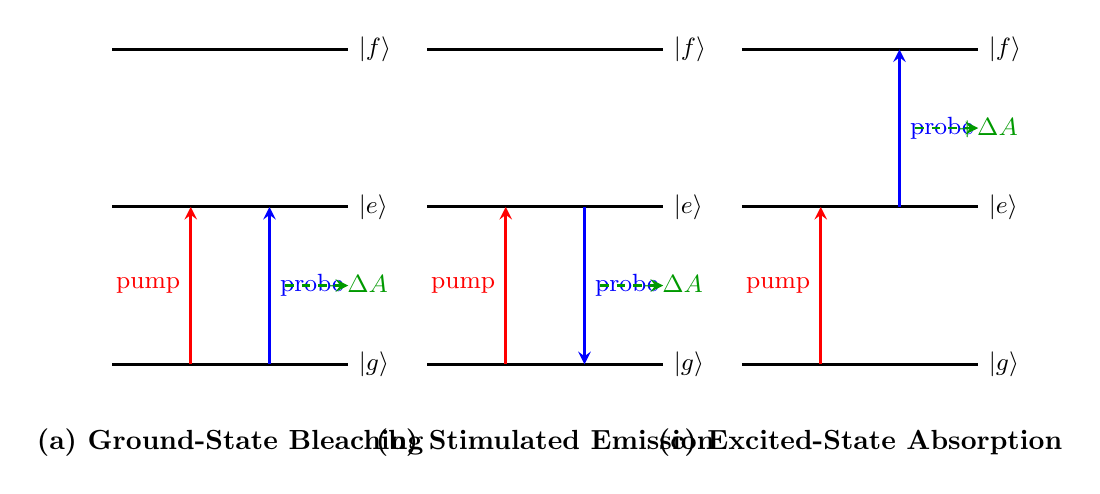
\begin{tikzpicture}[
        level/.style={thick, line width=1pt},
        arrow/.style={->, >=stealth, line width=1pt},
        pump/.style={arrow, red},
        probe/.style={arrow, blue},
        signal/.style={arrow, green!60!black, dashed},
        state/.style={font=\small\itshape},
        transition/.style={midway, font=\small},
        label/.style={font=\normalsize\bfseries}
    ]

    % Ground-State Bleaching (GSB)
    \begin{scope}[xshift=-4cm]
        % Energy levels
        \draw[level] (-1.5,0) -- (1.5,0) node[state,right] {$|g\rangle$};
        \draw[level] (-1.5,2) -- (1.5,2) node[state,right] {$|e\rangle$};
        \draw[level] (-1.5,4) -- (1.5,4) node[state,right] {$|f\rangle$};

        % Pump transition
        \draw[pump] (-0.5,0) -- (-0.5,2) node[transition, left] {pump};

        % Probe transition (reduced)
        \draw[probe] (0.5,0) -- (0.5,2) node[transition, right] {probe};

        % Signal (negative)
        \draw[signal] (0.7,1) -- (1.5,1) node[transition, right] {$-\Delta A$};

        % Title
        \node[label] at (0,-1) {(a) Ground-State Bleaching};
    \end{scope}

    % Stimulated Emission (SE)
    \begin{scope}[xshift=0cm]
        % Energy levels
        \draw[level] (-1.5,0) -- (1.5,0) node[state,right] {$|g\rangle$};
        \draw[level] (-1.5,2) -- (1.5,2) node[state,right] {$|e\rangle$};
        \draw[level] (-1.5,4) -- (1.5,4) node[state,right] {$|f\rangle$};

        % Pump transition
        \draw[pump] (-0.5,0) -- (-0.5,2) node[transition, left] {pump};

        % Probe stimulates emission
        \draw[probe] (0.5,2) -- (0.5,0) node[transition, right] {probe};

        % Signal (negative)
        \draw[signal] (0.7,1) -- (1.5,1) node[transition, right] {$-\Delta A$};

        % Title
        \node[label] at (0,-1) {(b) Stimulated Emission};
    \end{scope}

    % Excited-State Absorption (ESA)
    \begin{scope}[xshift=4cm]
        % Energy levels
        \draw[level] (-1.5,0) -- (1.5,0) node[state,right] {$|g\rangle$};
        \draw[level] (-1.5,2) -- (1.5,2) node[state,right] {$|e\rangle$};
        \draw[level] (-1.5,4) -- (1.5,4) node[state,right] {$|f\rangle$};

        % Pump transition
        \draw[pump] (-0.5,0) -- (-0.5,2) node[transition, left] {pump};

        % Probe transition (extra absorption)
        \draw[probe] (0.5,2) -- (0.5,4) node[transition, right] {probe};

        % Signal (positive)
        \draw[signal] (0.7,3) -- (1.5,3) node[transition, right] {$+\Delta A$};

        % Title
        \node[label] at (0,-1) {(c) Excited-State Absorption};
    \end{scope}

\end{tikzpicture}

\end{document}
